%=== CHAPTER TWO (2) ===
%=== Literature Review ===

\chapter{Literature Review}
\begin{spacing}{1.5}
\setlength{\parskip}{0.3in}

\section{Overview}

The main purpose of a literature review is to show the reader that the Student studied and analyzed viewpoints of other researchers on the problem under consideration. A literature review is not just a summary of the books read but rather a thorough analysis of other viewpoints on the problem being analysed. (2,000 – 4,000 words)


\section{One}
In euismod mauris tortor, non sodales tortor consectetur dapibus. Aenean dignissim ultricies lacus id malesuada. Cras laoreet luctus ligula, id dictum purus ultrices faucibus. Orci varius natoque penatibus et magnis dis parturient montes, nascetur ridiculus mus. Nulla at ante sed ex venenatis pretium in ut lorem. Cras condimentum pretium dignissim. Maecenas ac tempor ipsum, eu blandit enim. Mauris pharetra, justo in iaculis tincidunt, neque nisl eleifend tortor, in volutpat libero erat vitae lorem. Suspendisse dignissim quis eros eget varius. In porttitor augue vel ligula varius, a tincidunt eros gravida. Etiam eget porta ipsum.

Ut venenatis lectus at nisi consectetur volutpat. Vivamus vehicula a odio ac scelerisque. Fusce tincidunt diam eu orci pellentesque, eu vehicula felis posuere. Mauris tempus dignissim leo, vitae eleifend justo ultrices eget. Fusce volutpat suscipit urna. Curabitur ultrices nibh dolor, quis ultricies risus condimentum quis. Nulla non nulla quis odio laoreet pulvinar non eu turpis. Interdum et malesuada fames ac ante ipsum primis in faucibus. Morbi odio nisi, hendrerit id laoreet nec, fringilla quis neque. Quisque non nisl vitae leo vulputate fringilla. Sed blandit lectus dui, vestibulum tempor elit laoreet vel. Nullam at magna ut elit dapibus gravida vitae eu dolor. Aliquam ut odio ullamcorper, venenatis elit eget, feugiat arcu. Nunc nibh lacus, dapibus condimentum neque vitae, tempus eleifend ex. Integer sit amet volutpat orci, quis tristique augue. Nam sit amet dolor dignissim, luctus justo sit amet, luctus velit.

\begin{figure}[ht]
\centering
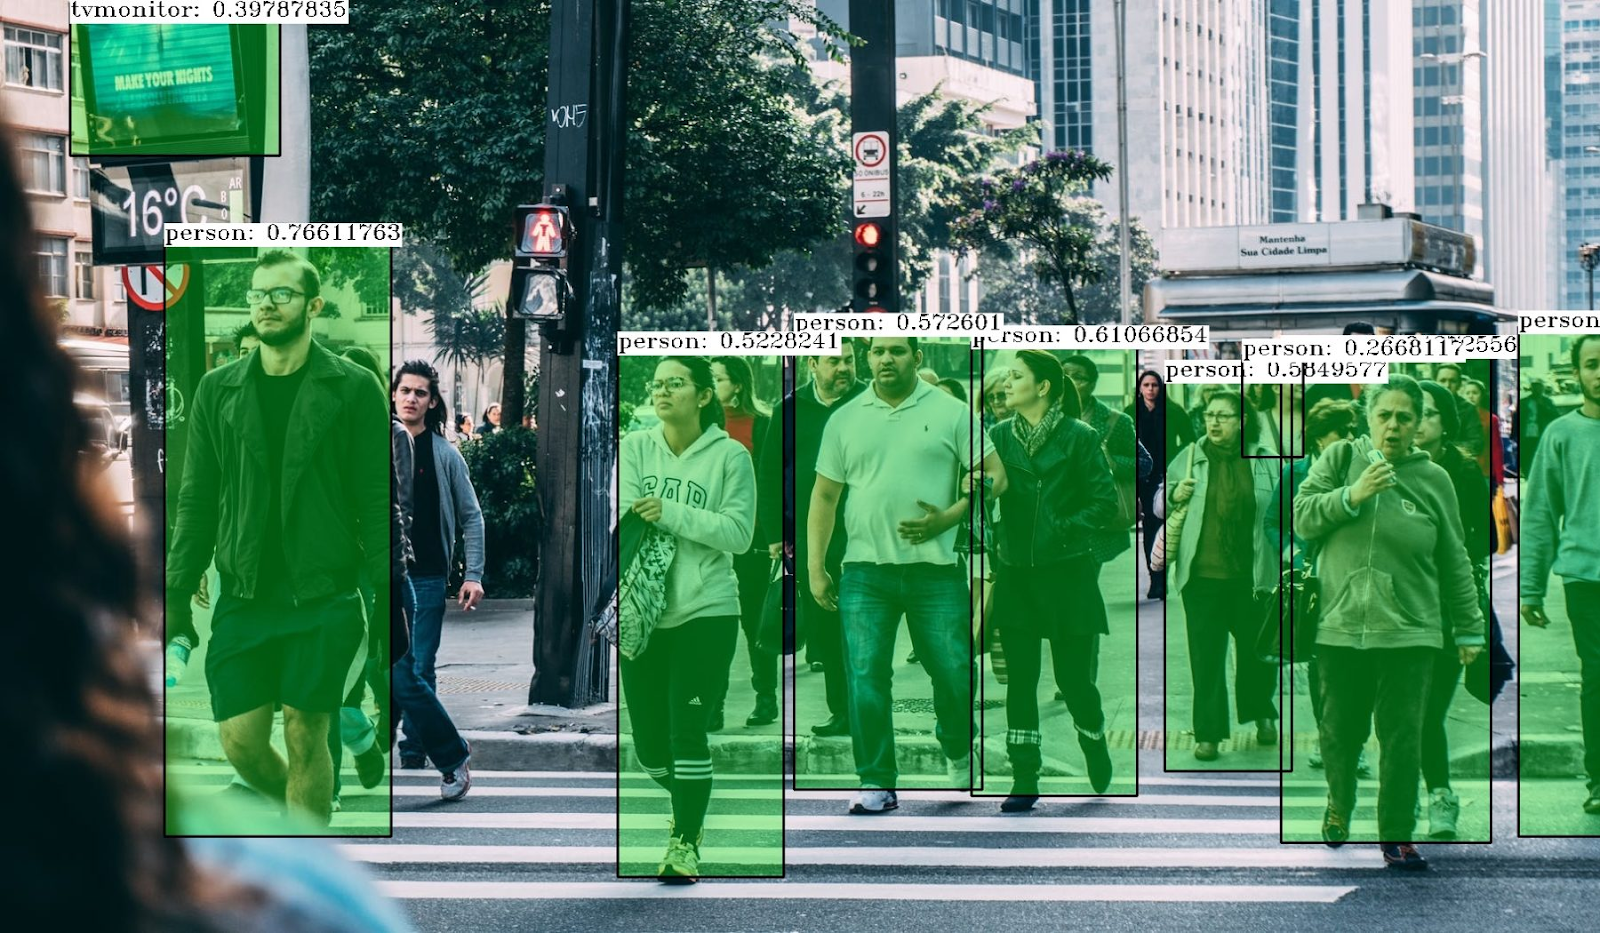
\includegraphics[width=5in, fbox]{Chapter1/opencv.png}
\caption{Machine Learning.}
\label{fig:opencvexample} 
\end{figure}

\section{Two}
In euismod mauris tortor, non sodales tortor consectetur dapibus. Aenean dignissim ultricies lacus id malesuada. Cras laoreet luctus ligula, id dictum purus ultrices faucibus. Orci varius natoque penatibus et magnis dis parturient montes, nascetur ridiculus mus. Nulla at ante sed ex venenatis pretium in ut lorem. Cras condimentum pretium dignissim. Maecenas ac tempor ipsum, eu blandit enim. Mauris pharetra, justo in iaculis tincidunt, neque nisl eleifend tortor, in volutpat libero erat vitae lorem. Suspendisse dignissim quis eros eget varius. In porttitor augue vel ligula varius, a tincidunt eros gravida. Etiam eget porta ipsum.

Ut venenatis lectus at nisi consectetur volutpat. Vivamus vehicula a odio ac scelerisque. Fusce tincidunt diam eu orci pellentesque, eu vehicula felis posuere. Mauris tempus dignissim leo, vitae eleifend justo ultrices eget. Fusce volutpat suscipit urna. Curabitur ultrices nibh dolor, quis ultricies risus condimentum quis. Nulla non nulla quis odio laoreet pulvinar non eu turpis. Interdum et malesuada fames ac ante ipsum primis in faucibus. Morbi odio nisi, hendrerit id laoreet nec, fringilla quis neque. Quisque non nisl vitae leo vulputate fringilla. Sed blandit lectus dui, vestibulum tempor elit laoreet vel. Nullam at magna ut elit dapibus gravida vitae eu dolor. Aliquam ut odio ullamcorper, venenatis elit eget, feugiat arcu. Nunc nibh lacus, dapibus condimentum neque vitae, tempus eleifend ex. Integer sit amet volutpat orci, quis tristique augue. Nam sit amet dolor dignissim, luctus justo sit amet, luctus velit.

\section{Three}
In euismod mauris tortor, non sodales tortor consectetur dapibus. Aenean dignissim ultricies lacus id malesuada. Cras laoreet luctus ligula, id dictum purus ultrices faucibus. Orci varius natoque penatibus et magnis dis parturient montes, nascetur ridiculus mus. Nulla at ante sed ex venenatis pretium in ut lorem. Cras condimentum pretium dignissim. Maecenas ac tempor ipsum, eu blandit enim. Mauris pharetra, justo in iaculis tincidunt, neque nisl eleifend tortor, in volutpat libero erat vitae lorem. Suspendisse dignissim quis eros eget varius. In porttitor augue vel ligula varius, a tincidunt eros gravida. Etiam eget porta ipsum.


\subsection{Four}
Ut venenatis lectus at nisi consectetur volutpat. Vivamus vehicula a odio ac scelerisque. Fusce tincidunt diam eu orci pellentesque, eu vehicula felis posuere. Mauris tempus dignissim leo, vitae eleifend justo ultrices eget. Fusce volutpat suscipit urna. Curabitur ultrices nibh dolor, quis ultricies risus condimentum quis. Nulla non nulla quis odio laoreet pulvinar non eu turpis. Interdum et malesuada fames ac ante ipsum primis in faucibus. Morbi odio nisi, hendrerit id laoreet nec, fringilla quis neque. Quisque non nisl vitae leo vulputate fringilla. Sed blandit lectus dui, vestibulum tempor elit laoreet vel. Nullam at magna ut elit dapibus gravida vitae eu dolor. Aliquam ut odio ullamcorper, venenatis elit eget, feugiat arcu. Nunc nibh lacus, dapibus condimentum neque vitae, tempus eleifend ex. Integer sit amet volutpat orci, quis tristique augue. Nam sit amet dolor dignissim, luctus justo sit amet, luctus velit.

%=== END OF CHAPTER TWO ===
\end{spacing}
\newpage
